%&LaTeX

\section{Working with J-DSP}

Welcome to the first Signal Computing lab! In this lab, I will introduce the
J-DSP system that we will be using for the bulk of our work in this
class. 
Note that this is intended to be an
\emph{orientation} to J-DSP. There's no way to do this without using
some digital signal processing vocabulary that you may not be familiar
with. However, you should not need to have a complete understanding of
these concepts to complete this lab. 

Note that these labs are divided into steps, with each step expecting a
response and numbered "X.Y". Step X.(Y+1) is based on step X.Y; in other
words, the instructions in step X.(Y+1) assume you are starting with the
J-DSP setup at the end of step X.Y; it modifies that setup. On the other
hand, step (X+1).1 starts with a completely new (blank) J-DSP workspace.

\subsection{General Information on J-DSP}

\begin{figure}
\begin{center}
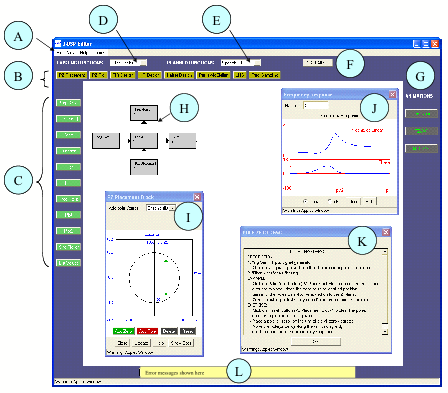
\includegraphics[width=0.75\textwidth]{lab1/simenv}
\end{center}
\caption{The J-DSP simulation environment. In the figure, A: Menu
  items; B: Filter blocks (this section changes according to the
  selection of D or E); C: Permanent blocks; D and E: List menu to
  select the group of functions; F: Disclaimer; G: Interactive visual
  demonstrations; H: Simulation flowgram; I: Dialog window
  (corresponding to the \block{PZ Placement} block in the block
  diagram H); J: Plot window to view the results; K: Help window
  provided for all the blocks; L: A field that shows error messages
  and warnings.\label{fg:simenv}}
\end{figure}

\begin{figure}
\begin{center}
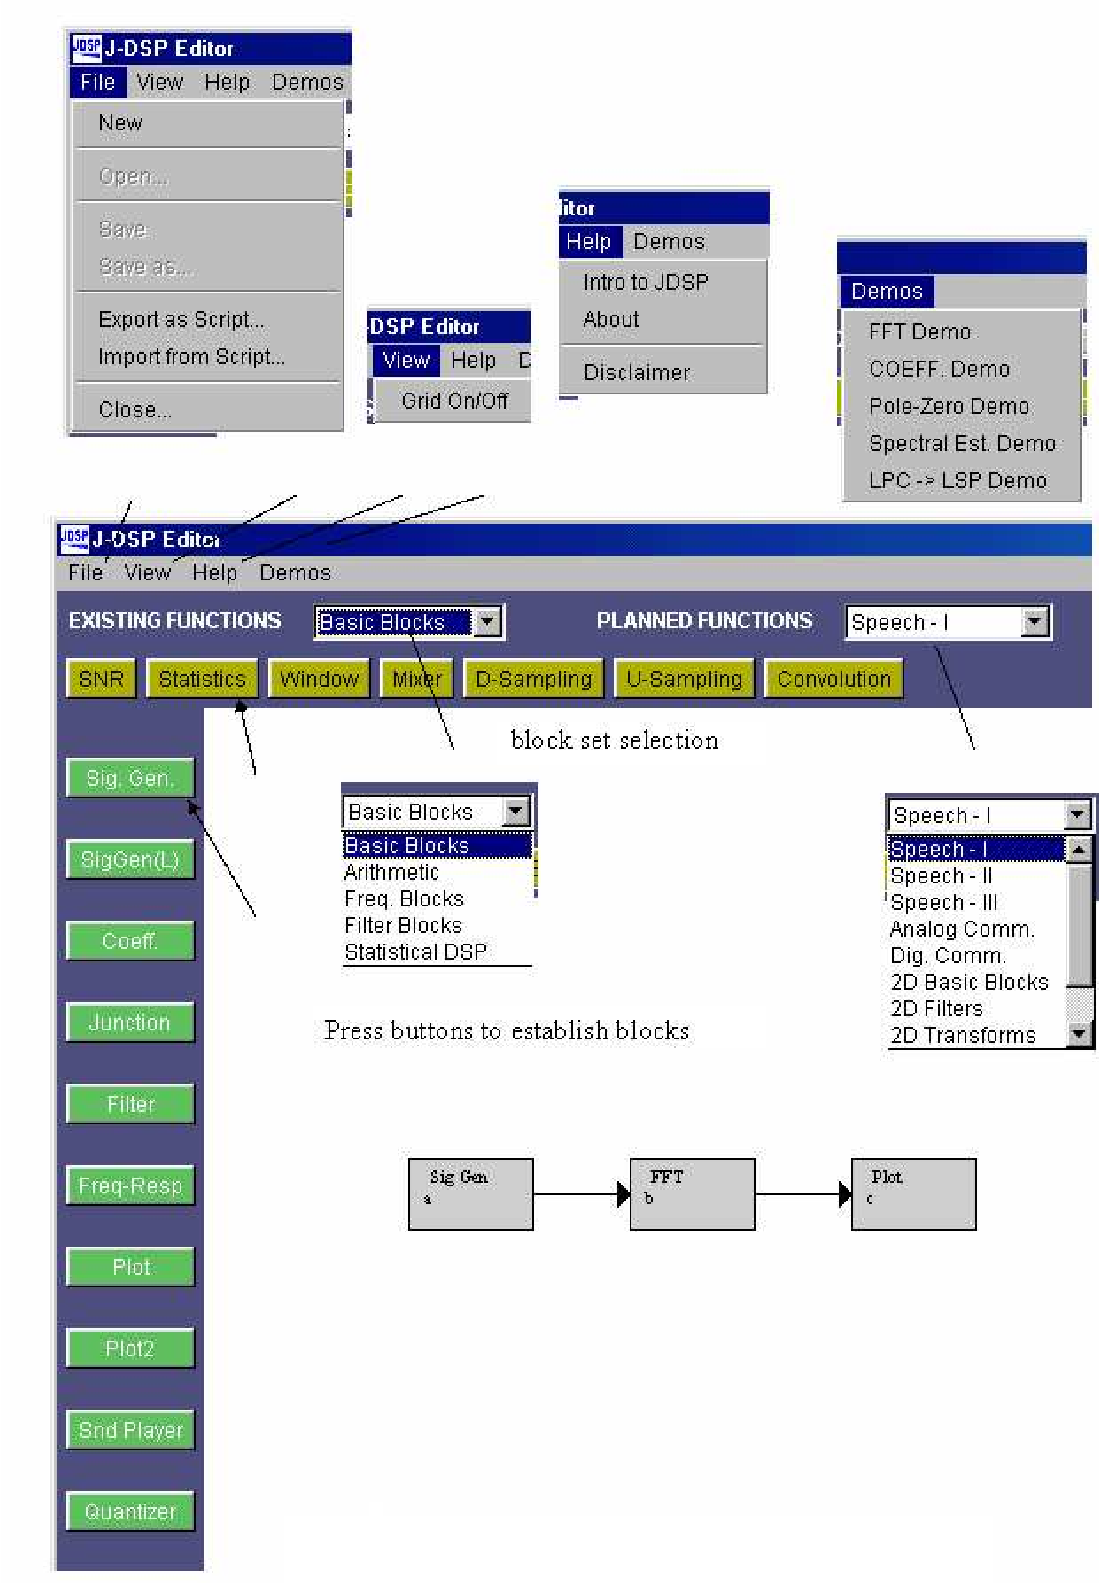
\includegraphics[height=0.5\textheight]{lab1/menus}
\end{center}
\caption{Signal processing functions and menus in J-DSP.\label{fg:menus}}
\end{figure}

All functions in J-DSP appear as graphical blocks that are divided
into groups according to their functionality. Selecting and
establishing individual blocks is done using a
drag-and-drop-process. Each block is linked to a signal processing
function. Figure~\ref{fg:simenv} shows the J-DSP editor environment
and Figure~\ref{fg:menus} shows details on the drop-down menus and the
signal processing functions of J-DSP. A simulation can be started by
connecting appropriate blocks from left to right. Signals at any point
of a simulation can be analyzed and plotted through the use of
appropriate functions. Parameters in the blocks can be edited through
dialog windows. Blocks can be manipulated easily (edit, move, delete
and connect) using the mouse. Execution is dynamic and therefore any
change at any point of a simulated system will automatically take
effect in all related blocks. Select windows can be left open to
enable viewing results at more than one point in the editor.

\subsection{Working with J-DSP}

Please note that the following notation has been used throughout the
laboratory assignments:
\begin{itemize}
\item Block names: bold and italic, e.g., \block{Plot}.
\item Drop down menu item name: bold, e.g., \menu{Basic Blocks}.
\item Button: brackets, e.g., \button{update}.
\item Option to be chosen by user in a dialog box: quotes, e.g.,
  \option{Gain}.
\end{itemize}

The easiest way to explain some of the functions of J-DSP is to work
through a simple example. To start J-DSP, go to
\href{http://depts.washington.edu/biocomp/J-DSP/}{http://depts.washington.edu/biocomp/J-DSP/},
click on ``Start J-DSP Locally'', and press ``Proceed'' in the
subsequent dialog window. This will load the applet; if you don't see
an applet with a ``Start!'' button, then there is a problem with Java
on your computer. Press the ``Start!'' button to open the J-DSP editor
window. When the start button is pressed and you attempt to establish
your first block a relatively large Java applet will start downloading
to the browser. Therefore it may take 30 seconds or more to establish
the first block for a telephone-based (28.8) internet connection but
once the first block is established the program should run reasonably
fast. Adjust the size of the J-DSP editor window so that you are able
to view the entire work area.

\begin{figure}
\begin{center}
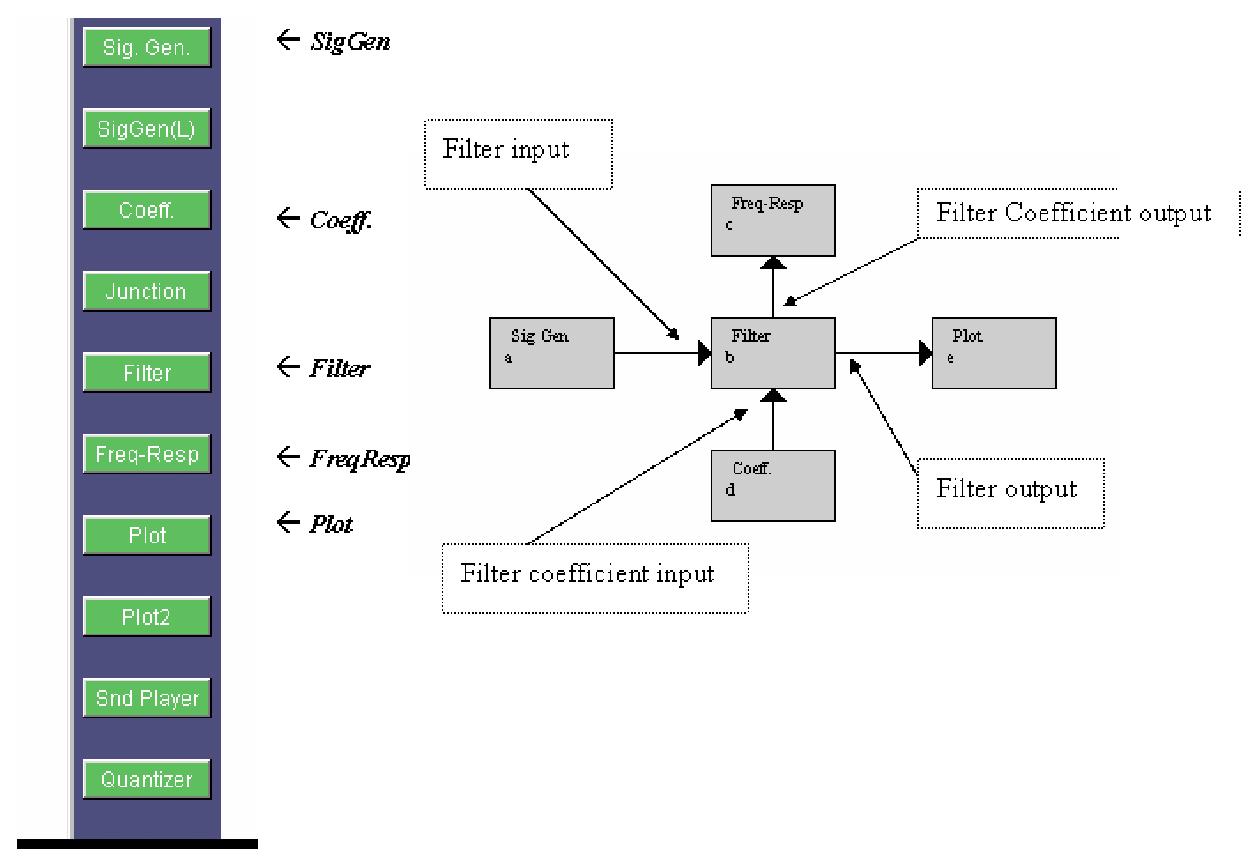
\includegraphics[width=0.75\textwidth]{lab1/buttons}
\end{center}
\caption{J-DSP buttons for a source-filter simulation.\label{fg:buttons}}
\end{figure}

Press the \block{SigGen} button on the left part of the window. Move
the mouse to the center of the window and click the left mouse button.
Note that you have created the signal generator block. There are two
signal generators, \block{SigGen} for processing a single frame of the
signal and \block{SigGen(L)} for frame-by-frame processing that is
typically used in speech processing simulations. Similarly, create
\block{Filter} and \block{Plot} blocks (their buttons are also on the
left) as in Figure~\ref{fg:buttons}. Note that blocks cannot be placed
on top of one another. There are two plot blocks, i.e., \block{Plot}
(single plot) and \block{Plot2} (two plots). For now, use
\block{Plot}.

Note that each block has signal input(s), designated by the small
triangular nodes, on the left and signal output(s) to the right. Some
blocks carry parameter inputs and outputs at the bottom and top of the
block respectively. For example, the \block{Filter} block has a
coefficient input on the bottom and a coefficient output on the
top. To select a block, click once to highlight it. You can then move
it by clicking and dragging it to a new location. Try this now with
your three blocks. To delete a block, simply select it and press the
``delete'' key on your keyboard. To link blocks, click once inside the
small triangle on the right side of one block and drag the cursor to a
triangle on the left side of another block. Release the mouse button
to create a connection between the two boxes. Do this now to connect
the output of the signal generator box to the input of the filter
box. Always make the connections in the direction of the signal flow.

\begin{figure}
\begin{center}
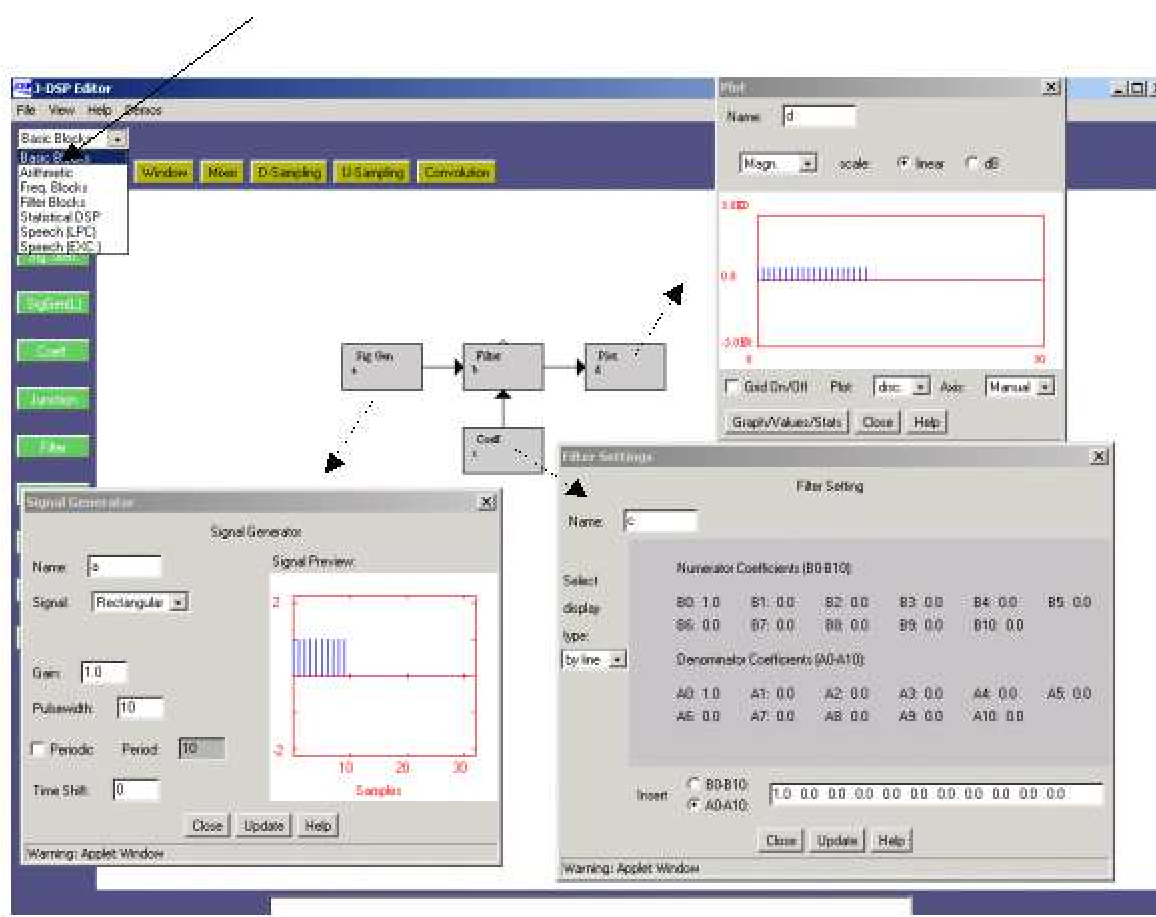
\includegraphics[width=0.75\textwidth]{lab1/image018}
\end{center}
\caption{Dialog windows in J-DSP.\label{fg:dialogs}}
\end{figure}

The \block{Coeff.} block is used to specify filter coefficients. The
block is connected to the \block{Filter} block parameter input as
shown in the figure; do so. Now, connect the \block{Filter} block to
the \block{Plot} block and add and connect a \block{Freq-Resp} block
(buttons for both are on the left) so that your editor window looks
like the block diagram. Note that you can view the dialog box of each
block by double-clicking on the block, as shown in
Figure~\ref{fg:dialogs}.

\subsection{Choosing Signals}

\begin{figure}
\begin{center}
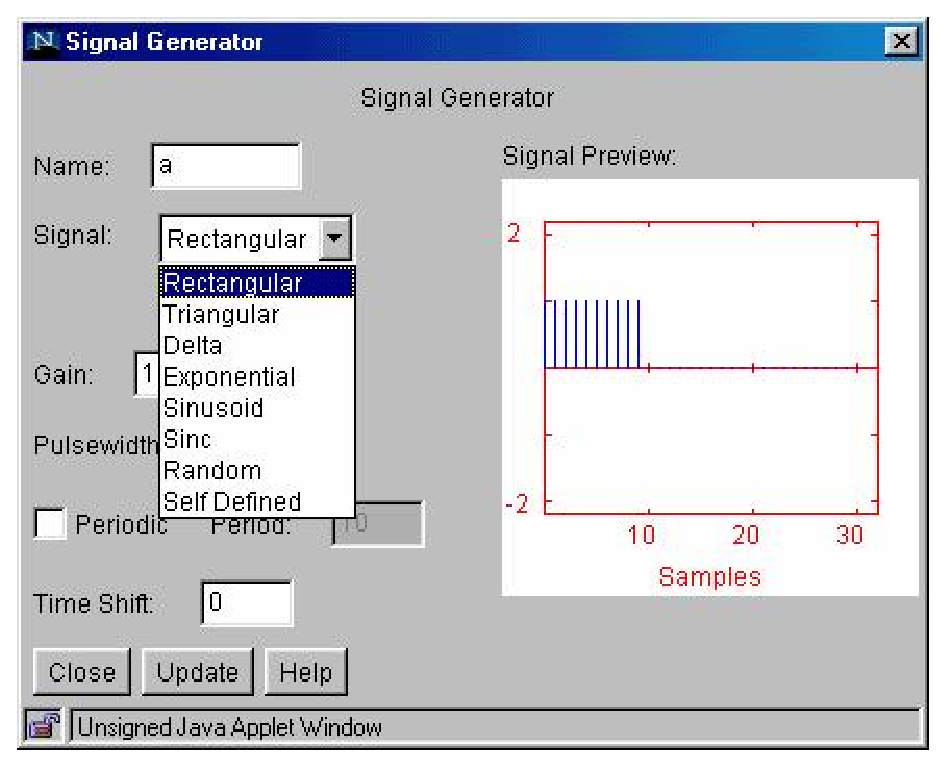
\includegraphics[width=0.5\textwidth]{lab1/image020}
\end{center}
\caption{Signal generator dialog.\label{fg:sig-gen}}
\end{figure}

Let us now form a signal using the signal generator. Double click
the \block{Sig Gen} box and a dialog window will
appear, Figure~\ref{fg:sig-gen}. If you do not see a dialog window,
your browser may be too old a version to work with J-DSP.

On the right side of the signal generator window, you can see a
preview of part of the signal. You may change the \option{name} of the
signal, the \option{gain} (the signal amplitude is $\pm$gain), the
\option{pulse width} (the number of samples in the entire signal), the
\option{period} and the \option{time shift} by typing the desired
value into the appropriate box. The signal type can be changed by
clicking on the pull-down menu and selecting a signal. If you select a
User-defined signal, an [Edit signal] button will appear allowing you
to edit the signal. With all signals except audio, J-DSP assumes a
normalized sampling frequency of 1Hz. Hence the sampling frequency in
terms of radians is $2\pi$. (Don't worry about these details right
now; this will become clear after we cover ``Signals in the
Computer,'' chapter~2 of the course notes.) All frequencies are
entered as a function of $\pi$, e.g., $0.1\pi$, $0.356\pi$, etc. Any
sinusoidal frequency at or above $\pi$ will result in \emph{aliasing}
(again, this will be explained in chapter~2 of the course notes).

\paragraph{Step 1.1} Create a sinusoid with \option{frequency}
$0.1\pi$, \option{gain} 3.75, \option{pulsewidth} 40. When all of the
parameters have been entered, press the \button{update} button to
update the signal preview. Remember that whenever changes are made to
this box, the \button{update} button must be pressed in order for the
changes to take effect. On the right, you can see a preview of the
input signal. Note that the vertical range (or ``peak-to-peak
amplitude'') of the signal is twice the \option{gain}, or
$\pm$gain. In these laboratories, unless otherwise indicated, we will
use ``amplitude'' as a synonym for the signal generator \option{gain}
and so, for a $\pm3.75$ signal, we will say it has an ``amplitude'' of
3.75.  Include an image of your block diagram in your lab
writeup. Count the number of samples (vertical bars) within a period
of the sinusoid. Don't forget that there are zero-height bars where
the amplitude of the sinusoid is zero. How many do you have?

\paragraph{Step 1.2} Create a sinusoid with \option{frequency} $\pi$,
\option{gain} 3.75, \option{pulse width} 40 (remember to press
update for changes to take place). What happens?

\paragraph{Step 1.3} Create a sinusoid with \option{frequency}
$1.3\pi$, \option{gain} 3.75, \option{pulse width} 40. What
happens? 


\subsection{Viewing Signals}

\paragraph{Step 2} Next, we want to take a look at the \block{Filter}
output in the time and frequency domain. Set the values in \block{Sig
  Gen} as per step 1.1.  Double-click the \block{Plot} block and a new
dialog window will appear. You should again see the input signal
because the filter is just letting the signal pass through unaffected,
since no coefficients have been set. If you move the mouse cursor
within the plot, cross hairs will appear and the $(x,y)$ coordinate at
the cross hair ``target'' will be displayed. If you press the
\button{Graphs/Values/Stats} button, a table with the values of the
signal pops up. In the first column you see the indices of the samples
and the second column shows you the values.  Press the
\button{Graphs/Values/Stats} button again to see a summary of some of
the signal statistics. A third press will return us to the graph.

\begin{figure}
\begin{center}
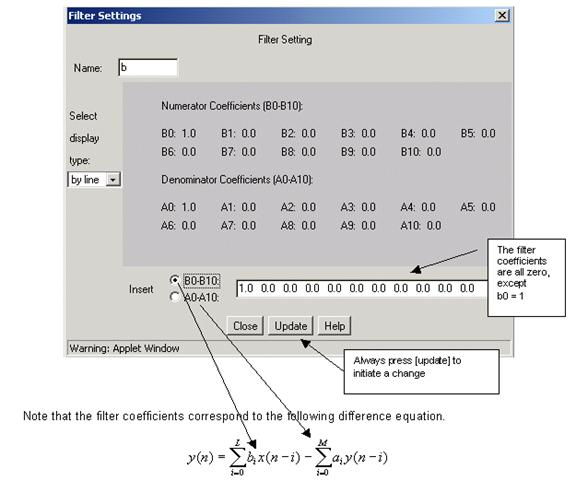
\includegraphics[width=0.75\textwidth]{lab1/image022}
\end{center}
\caption{Coefficient entry in J-DSP.\label{fg:coef-entry}}
\end{figure}

\paragraph{Step 2.1} Let us now see the filter in action. Keep the
\block{Plot} window open to observe any changes. Double click the
\block{Coeff.} block. You should see the display in
Figure~\ref{fg:coef-entry}.

\paragraph{Step 2.2} Keep the values in \block{Sig Gen} as per step
1.1. Change the filter coefficient to $b_0=4$ (it will probably be
easier to set the \option{display type} to ``tabular'' for setting the
coefficients) and press \button{update}. Include an image of your
block diagram and open block parameter and display windows in your
writeup. Look in the plot window. You should see that the amplitude of
the sinusoid has changed. What is it now?


\paragraph{Step 2.3} Implement a pure delay by setting $b_5=1$ and
rest of the coefficients (including $b_0$) to zero and press
\button{update}. Remember to verify after you press \button{update}
that you correctly set the desired coefficients. Include an image of
your block diagram and open block parameter and display windows in
your writeup. What happens to the sinusoid?


\paragraph{Step 2.4} Implement a simple ``low pass filter'' by setting
$b_0=0.2$ and $a_1=-0.8$ (reset $b_5$ to zero) and pressing
\button{update}.  Generate a sinusoid with \option{gain} 1,
\option{frequency} $0.1\pi$, \option{pulse width} 256. Include an
image of your block diagram and open block parameter and display
windows in your writeup. What do you observe?  What kind of signal do
you get at the output? What is the peak-to-peak value?


\paragraph{Step 2.5} Select the \block{Freq-Resp} block from the panel
of general blocks on the left of the window and place it to the north
of the \block{Filter} block. Connect the parameter output to the
\block{Freq-Resp} block. Double click the \block{Freq-Resp} block. You
should see the magnitude and phase response of the filter. Change the
coefficient to $a_1 = 0.8$ instead of $a_1 = -0.8$. Include an image
of your block diagram and open block parameter and display windows in
your writeup. What do you see in the frequency response (the magnitude
plot) and output?


\begin{figure}
\begin{center}
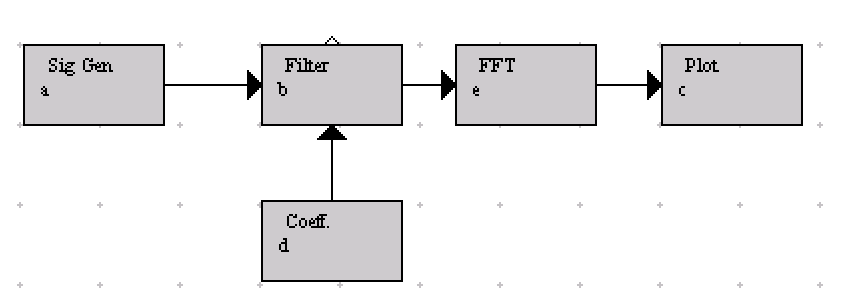
\includegraphics[width=0.75\textwidth]{lab1/image023}
\end{center}
\caption{Source-filter simulation with FFT at the output.\label{fg:sim}}
\end{figure}

\paragraph{Step 3} To view the signal in the frequency domain, insert
an \block{FFT} block between the \block{Filter} and the \block{Plot}
box as shown in Figure~\ref{fg:sim}. The \block{FFT} box can be found
in the column of buttons on the left or under ``Freq. Blocks'' in the
\menu{Existing Functions} menu.

\paragraph{Step 3.1} Set the \block{Filter} parameters and input as
per step 2.4. Double click on the \block{FFT} block and change the
\option{FFT size} to 256 points and then press \button{Update} and
\button{Close}. Now, you can see the amplitude of the signal in the
frequency domain. The magnitude has a sharp peak approximately at
0.31, the frequency of our sinusoidal signal ($0.1 \times
3.1459$). Include an image of your block diagram and open block
parameter and display windows in your writeup.

\paragraph{Step 3.2} Change the sinusoidal frequencies \emph{only} as
per steps 1.2 and 1.3 but with \option{pulse width} 256. Include an
image of your block diagram and open block parameter and display
windows in your writeup. What do you observe?


\begin{figure}
\begin{center}
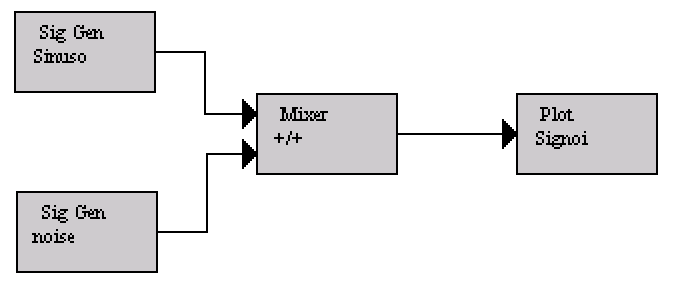
\includegraphics[width=0.75\textwidth]{lab1/image024}
\end{center}
\caption{Sinewave plus noise simulation.\label{fg:sin-noise}}
\end{figure}

\paragraph{Step 3.3} Delete the \block{Filter} and \block{Coef}. Set
the sinusoidal \option{frequency} in \block{Sig Gen} as per step 1.1
but with \option{pulse width} 256. Now create a second \block{Sig Gen}
block and a \option{Mixer} block (use the \button{Adder} button under
\menu{Basic Blocks}). Your editor window should then look
like Figure~\ref{fg:sin-noise}.

Change the name of the first \block{Sig Gen} block to `Sinusoi', the
second \block{Sig Gen} block to `noise' and the \block{Plot} block to
`SigNoi'. The names are restricted to six characters. Following that,
we edit the \block{Sig Gen} block called `noise'. Open the dialog
window and change the \option{signal type} to \option{random}. Choose
a \option{variance} of 4 and extend the \option{pulse width} to 256
samples, in order to have noise over the full length of the
signal. Now take a look at the output signal. In the time domain it is
very hard to see that a sinusoid is present.  However, if you view the
signal in the frequency domain with an FFT size of 256, then you still
find a peak at approximately 0.31.

\paragraph{Step 3.4} Change the amplitude of the sinusoid up or down
and observe the spectra (FFT plot). Try different values to make the
sinusoid dominate the noise signal or be masked by the noise
signal. Remember the movie ``The Hunt for Red October'' which was
about a stealth Soviet submarine defecting? In that movie they showed
sonar operators viewing FFT spectra and listening to sonar signals as
they were searching for submarine propeller signatures (quasi-periodic
signals) in ocean noise (random broadband signals). Stealth submarines
have, among other things, weak broadband propeller signatures that can
be masked easily by ocean noise.

\subsection{Submitting Your Work}

Please submit a lab writeup as requested by your instructor. Think of
this as being a report documenting your actions, observations, and
conclusions from your lab work. Thus, in responding to a question
like, ``what do you observe?'', you might comment on the major
features of a plot, such as the $Y$ values of typical points, the
range of $Y$ values overall, the number of points in the graph,
overall shape, comparison of extreme values' $X$ and $Y$ coordinates
to other values', etc. If you're asked something like, ``what can you
conclude?'', you would make the above observations and then use that
information to produce a conclusion such as, ``When I set the filter
coefficient, the noise peak is reduced by a factor of 10''.

